% !TEX root = sum1.tex
\section{Computational Experiments}\label{sec_result}
We conduct several experiments, including analyzing the performances of different policies, evaluating the impact of implementing social distancing, and comparing the performance under varied constraints.
In the experiments, we set the following parameters. 

The default parameters in the experiments are as follows, the size of social distancing $\delta =1$, the largest group size $M =4$, the number of rows $N = 10$, and the size of each row $L_j = 21$, for all $j \in \mathcal{N}$. We simulate the arrival of exactly one group in each period, i.e., $p_0 = 0$. Each experiment result is the average of 100 instances. In each instance, the number of scenarios in SBSP is $|\Omega| = 1000$.

To assess the performances of different policies across varying demand levels, we conduct experiments spanning a range of 60 to 100 periods and we consider four probability distributions for our analysis: $D_1:[0.18,0.7,0.06,0.06]$ and $D_2:[0.2,0.8,0,0]$, $D_3: [0.34, 0.51, 0.07, 0.08]$ and $D_4: [0.12, 0.5, 0.13, 0.25]$. The first two distributions, $D_1$ and $D_2$, are experimented in \cite{blom2022filling}. Here, $D_1$ represents the statistical distribution of group sizes, while $D_2$ reflects a restricted situation where groups of more than 2 people are not allowed. The other two distributions, $D_3$ and $D_4$, are derived from real-world movie data. The specific procedure is detailed in Appendix \ref{appen_3}. We use $D_4$ as the default probability distribution in the other experiments.

% Specifically, we select Movie A (representing the suspense genre) and Movie B (representing the family fun genre) as target movies to analyze group information and their corresponding probability distributions, denoted as $D3$ and $D4$, respectively. The seat plans for the tickets were obtained from a Hong Kong cinema website. We focused on scattered seat plans and excluded cases where the number of consecutive seats exceeded four. By counting the occurrences of different group types, we obtained these distributions. 

\subsection{Performances of Different Policies}
We evaluate four assignment policies: seat-plan-based assignment (SPBA), relaxed dynamic programming heuristic (RDPH), bid-price control (BPC), and booking-limit control (BLC), comparing their performance against the optimal policy derived by solving the deterministic model with perfect information of all requests. Table \ref{tab_perf} compares their effectiveness using the ratio of accepted individuals under each policy to those accepted under the optimal policy.


\begin{table}[h]
  \centering
  \caption{Performances of Different Policies}\label{tab_perf}
  \begin{tabular}{cccccc}
  \hline
  Distribution & T & SPBA (\%) & RDPH (\%) & BPC (\%) & BLC (\%) \\
  % \Xcline{1-1}{0.4pt}\Xcline{3-3}{0.4pt}\Xcline{4-4}{0.4pt}
  % \cmidrule(r){0-1} \cmidrule(lr){3-3} \cmidrule(lr){4-4} \cmidrule(lr){5-5} \cmidrule(lr){6-6} \cmidrule(l){7-7}
  \hline
  \multirow{5}{*}{$D_1$} & 60 & 100.00 & 100.00 & 100.00 & 88.56 \\
  & 70    & 99.53 & 99.01 & 98.98 & 92.69  \\
  & 80    & 99.38 & 98.91 & 98.84 & 97.06  \\
  & 90    & 99.52 & 99.23 & 99.10 & 98.24  \\
  & 100   & 99.58 & 99.27 & 98.95 & 98.46 \\
  \hline
  \multirow{5}{*}{$D_2$} & 60  & 100.00 & 100.00 & 100.00 & 93.68  \\
     & 70  & 100.00 & 100.00 & 100.00 & 92.88  \\
     & 80  & 99.54 & 97.89 & 97.21 & 98.98  \\
     & 90  & 99.90 & 99.73 & 99.44 & 99.61  \\
     & 100 & 100.00 & 100.00 & 100.00 & 99.89  \\ 
  \hline
  \multirow{5}{*}{$D_3$} & 60  & 100.00 & 100.00 & 100.00 & 91.07  \\
  & 70  & 99.85 & 99.76 & 99.73 & 90.15 \\
  & 80  & 99.22 & 98.92 & 98.40 & 96.98  \\
  & 90  & 99.39 & 99.12 & 98.36 & 96.93  \\
  & 100  & 99.32 & 99.18 & 98.88 & 97.63  \\
    \hline
    \multirow{5}{*}{$D_4$} & 60  & 99.25 & 99.18 & 99.13 & 93.45  \\
     & 70  & 99.20 & 98.65 & 98.54 & 97.79  \\
     & 80  & 99.25 & 98.69 & 98.40 & 98.22 \\
     & 90  & 99.29 & 98.65 & 98.02 & 98.42  \\
     & 100 & 99.60 & 99.14 & 98.32 & 98.68 \\
  \hline
  \end{tabular}
\end{table}

Our results demonstrate that the SPBA policy consistently outperforms the RDPH, BPC and BLC policies. The RDPH and BPC policies can make the initial decision to accept or reject a request, but lack the capability to optimize seat assignments. The BLC policy strictly adheres to predetermined booking limits; even if the supply of one type is exhausted, it does not utilize seats planned for other types to accept the request, leading to its limited effectiveness.

The performance of SPBA, RDPH, and BPC policies basically follows a pattern where it initially declines and then gradually improves as $T$ increases. When $T$ is small, the demand of requests is generally low, allowing these policies to achieve relatively optimal performance. However, as $T$ increases, it becomes more challenging for these policies to consistently achieve a perfect allocation, resulting in a decrease in performance. Nevertheless, as $T$ continues to grow, these policies tend to accept larger groups, thereby narrowing the gap between their performance and the optimal value. Consequently, their performances improve. In contrast, the BLC policy shows improved performance as $T$ increases because it reduces the number of unoccupied seats reserved for the largest groups. 

The performance of the policies can vary with different probabilities. For the different probability distributions listed, the SPBA policy performs more stably and consistently for the same demand. In contrast, the performances of the other policies fluctuate more significantly.


\subsection{Impact of Social Distancing}\label{impact_sd}
We introduce three key terms, the threshold of request-volume, the threshold of occupancy rate, and the maximum achievable occupancy rate, to describe the impact of implementing social distancing.

The \textit{threshold of request-volume}, ${q}^{\textup{th}}$, is defined as 
\[
{q}^{\textup{th}} = (1- p_0) \cdot \max\left\{T \,\bigg|\, E^{0}(T) - E(T) < 1\right\},
\]
where $E(T)$ and $E^{0}(T)$ denotes the average number of accepted individuals by SPBA with social distancing level $\delta$ and without social distancing, respectively. Here, the maximization is performed over $T$ while keeping all other parameters constant.
Intuitively, the threshold of request-volume represents the maximum number of requests that can be accommodated while keeping the average loss below one.


The occupancy rate corresponding to the threshold of request-volume is referred to as the \textit{threshold of occupancy rate}, $\rho^{\textup{tr}}$. This rate represents the maximum occupancy rate when the difference in the number of accepted individuals remains unaffected by the social distancing requirement.

The \textit{maximum achievable occupancy rate} is attained when each row of a given layout is the largest pattern, denoted by $\rho^{ac} = \frac{\sum_{j \in \mathcal{N}}\phi(M, L_{j}^{0}, \delta)}{\sum_{j \in \mathcal{N}} L_{j}^{0}}$, as introduced in Section \ref{seat_planning_full_largest}.

We examine the impact of social distancing when implementing SPBA under varying levels of demand.  Specifically, we calculate $E(T)$ with $\delta = 1$ and $E^{0}(T)$ across different values of $T$. The demand levels are varied by adjusting the parameter $T$ from 40 to 100 in increments of 1. The results are visualized in Figure \ref{occupancy_rate_demand}, which illustrates the occupancy rate under different demand levels.

% By analyzing and comparing the data, we can gain insights into the relation between demand, social distancing, the number of accepted individuals, and occupancy rates. This information is valuable for understanding the impact of social distancing policies on overall capacity utilization and making informed decisions regarding resource allocation and operational strategies.


\begin{figure}[h]
  \centering
  \subfigure[]{
    \label{x_period}
    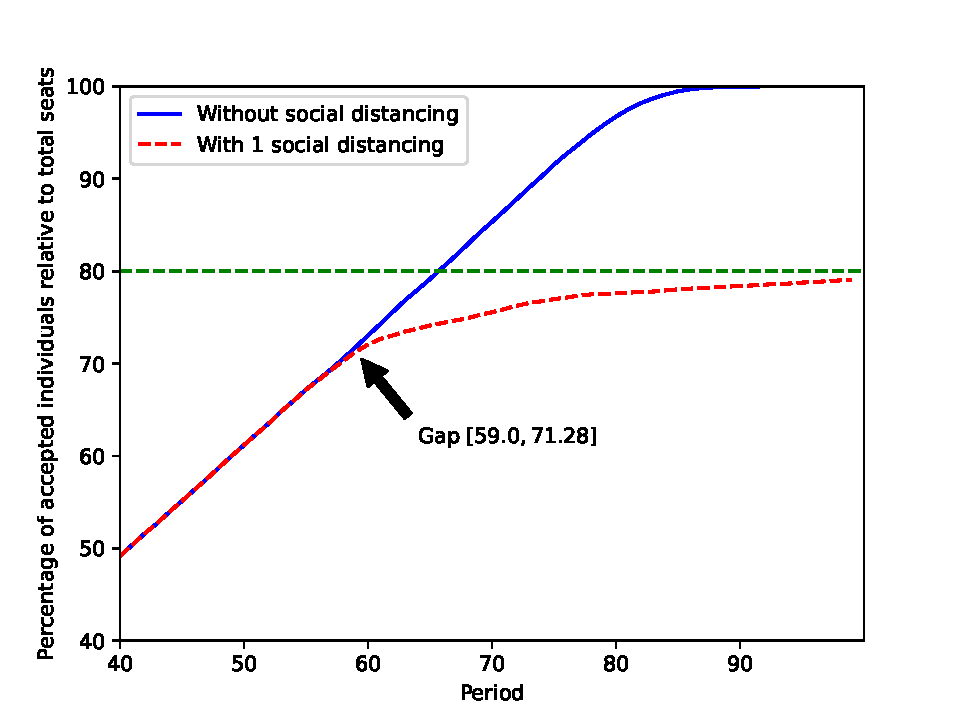
\includegraphics[width=0.48\textwidth]{./Figures/occu_demand_group4.pdf}}
    \subfigure[]{
      \label{x_demand}
      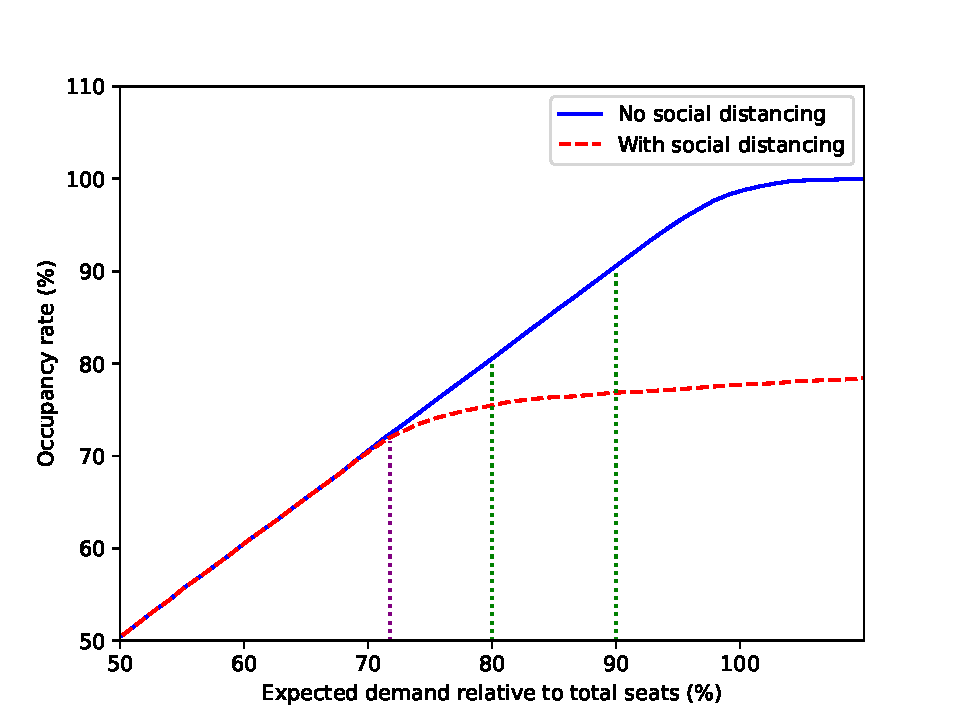
\includegraphics[width=0.48\textwidth]{./Figures/occu_gamma_group4.pdf}}
      \caption{Impact of Social Distancing}\label{occupancy_rate_demand}
\end{figure}


Figure \ref{x_period} illustrates the occupancy rate over period, revealing three key metrics for policy evaluation: (1) the threshold of request-volume, ${q}^{\textup{th}} = 57$, (2) the threshold of occupancy rate, $\rho^{th} = 71.8\%$, and (3) the maximum achievable occupancy rate $\rho^{ac} =80\%$. These metrics collectively serve as crucial indicators for assessing the effectiveness of the government policy.


% The above qualitative insights are stable concerning the tightness of the policy as well as the specific characteristics of various venues.
% Based on the above analysis, we also explore the results of different layouts, different group sizes and different social distances. 

% Since the figure about the occupancy rate over demand is similar to Figure \ref{occupancy_rate_demand}, we only use three metrics to show the results: the threshold of requests and the threshold occupancy rate, the maximum achievable occupancy rate.


Figure \ref{x_demand} presents the occupancy rate as a function of expected demand. The key distinction between Figure \ref{x_period} and Figure \ref{x_demand} lies in their respective x-axes. From a demand perspective, we observe two distinct points: for expected demand below 71.8\%, social distancing requirements impose no significant reduction in the number of accepted individuals; above this 71.8\% threshold, the performance gap between scenarios with and without social distancing becomes increasingly pronounced.

Given the conceptual similarity between period-based and demand-based occupancy rate analyses, we focus on these three metrics to concisely represent the core findings. Complete results and detailed interpretations are presented in Section \ref{perf_constraints}, which examines performance under various policy constraints.


\subsection{Estimation of $q^{th}$ and $\rho^{th}$}
To estimate the threshold of request-volume, we aim to find the maximal period such that all requests can be assigned into the seats during these periods, i.e., for each group type $i$, we have $\bm{X}_{i} = \sum_{j} x_{ij} \geq d_i$. Meanwhile, we have the capacity constraint $\sum_{i} n_{i} x_{ij} \leq L_j$, thus, $\sum_{i} n_i d_i \leq \sum_{i} n_i \sum_{j} x_{ij} \leq \sum_{j} L_{j}$. Notice that $E(d_i) = p_i T$, we have $\sum_{i} n_i p_i T \leq \sum_{j} L_{j}$ by taking the expectation. The average number of individuals per period, denoted as $\gamma$, can be expressed as $\gamma = \sum_{i=1}^{M} i p_i$. Recall that $\tilde{L} = \sum_{j} L_{j}$ denotes the total size of all rows. From this, we derive the inequality $T \leq \frac{\tilde{L}}{\gamma + \delta}$. Under the ideal assumption that all requests fully occupy the available capacity, the ideal threshold of request-volume can be estimated as $\hat{q}^{\textup{th}} = (1-p_0) \frac{\tilde{L}}{\gamma + \delta}$. Correspondingly, the threshold of occupancy rate under this ideal scenario is: 
$\hat{\rho}^{\textup{th}}= \frac{\gamma \hat{q}^{\textup{th}}}{(\gamma+ \delta)\hat{q}^{\textup{th}} - N \delta} = \frac{\gamma}{\gamma +\delta} \frac{(1-p_0) \tilde{L}}{(1-p_0) \tilde{L}-N \delta}$. 


However, in practice, the actual expected maximum request-volume will be smaller than $\hat{q}^{\textup{th}}$ since perfectly filling all available capacity is nearly impossible. To account for this, we introduce discount factors $c_1$ and $c_2$ for both thresholds, respectively. For the threshold of request-volume:
$\tilde{q}^{th} =  \frac{c_1 (1-p_0) \tilde{L}}{\gamma + \delta}$, where $c_1$ adjusts for deviations from the ideal assumption.
For the threshold of occupancy rate:
$\tilde{\rho}^{th} = \frac{c_2 \gamma}{\gamma +\delta} \frac{(1-p_0) \tilde{L}}{(1-p_0) \tilde{L}-N \delta}$, where $c_2$ similarly reflects practical constraints.

To analyze the relation between the threshold of request-volume, the threshold of occupancy rate and $\gamma$, we conducted a study using a sample of 200 probability distributions with $M=4, p_0=0$. The figure below shows the threshold of request-volume and the threshold of occupancy rate as functions of $\gamma$, along with their corresponding estimations.

We applied an Ordinary Least Squares model to fit the data and estimate the parameters. The resulting fitted equations, $\tilde{q}^{th} = \frac{c_1 \tilde{L}}{\gamma + \delta}$ (represented by the solid line in the figure) and $\tilde{\rho}^{th} = \frac{c_2 \gamma}{\gamma + \delta} \frac{\tilde{L}}{\tilde{L}-N \delta}$ (represented by the dashed line in the figure), are displayed in the figure. The goodness of fit is evaluated using R-squared values, which are 1.000 for both models, indicating a perfect fit between the data and the fitted equations. The estimated discount factor values are $c_1 = 0.9578$ and $c_2 = 0.9576$.

\begin{figure}[ht]
  \caption{The estimations of threshold of request-volume and occupancy rate}
  \centering
    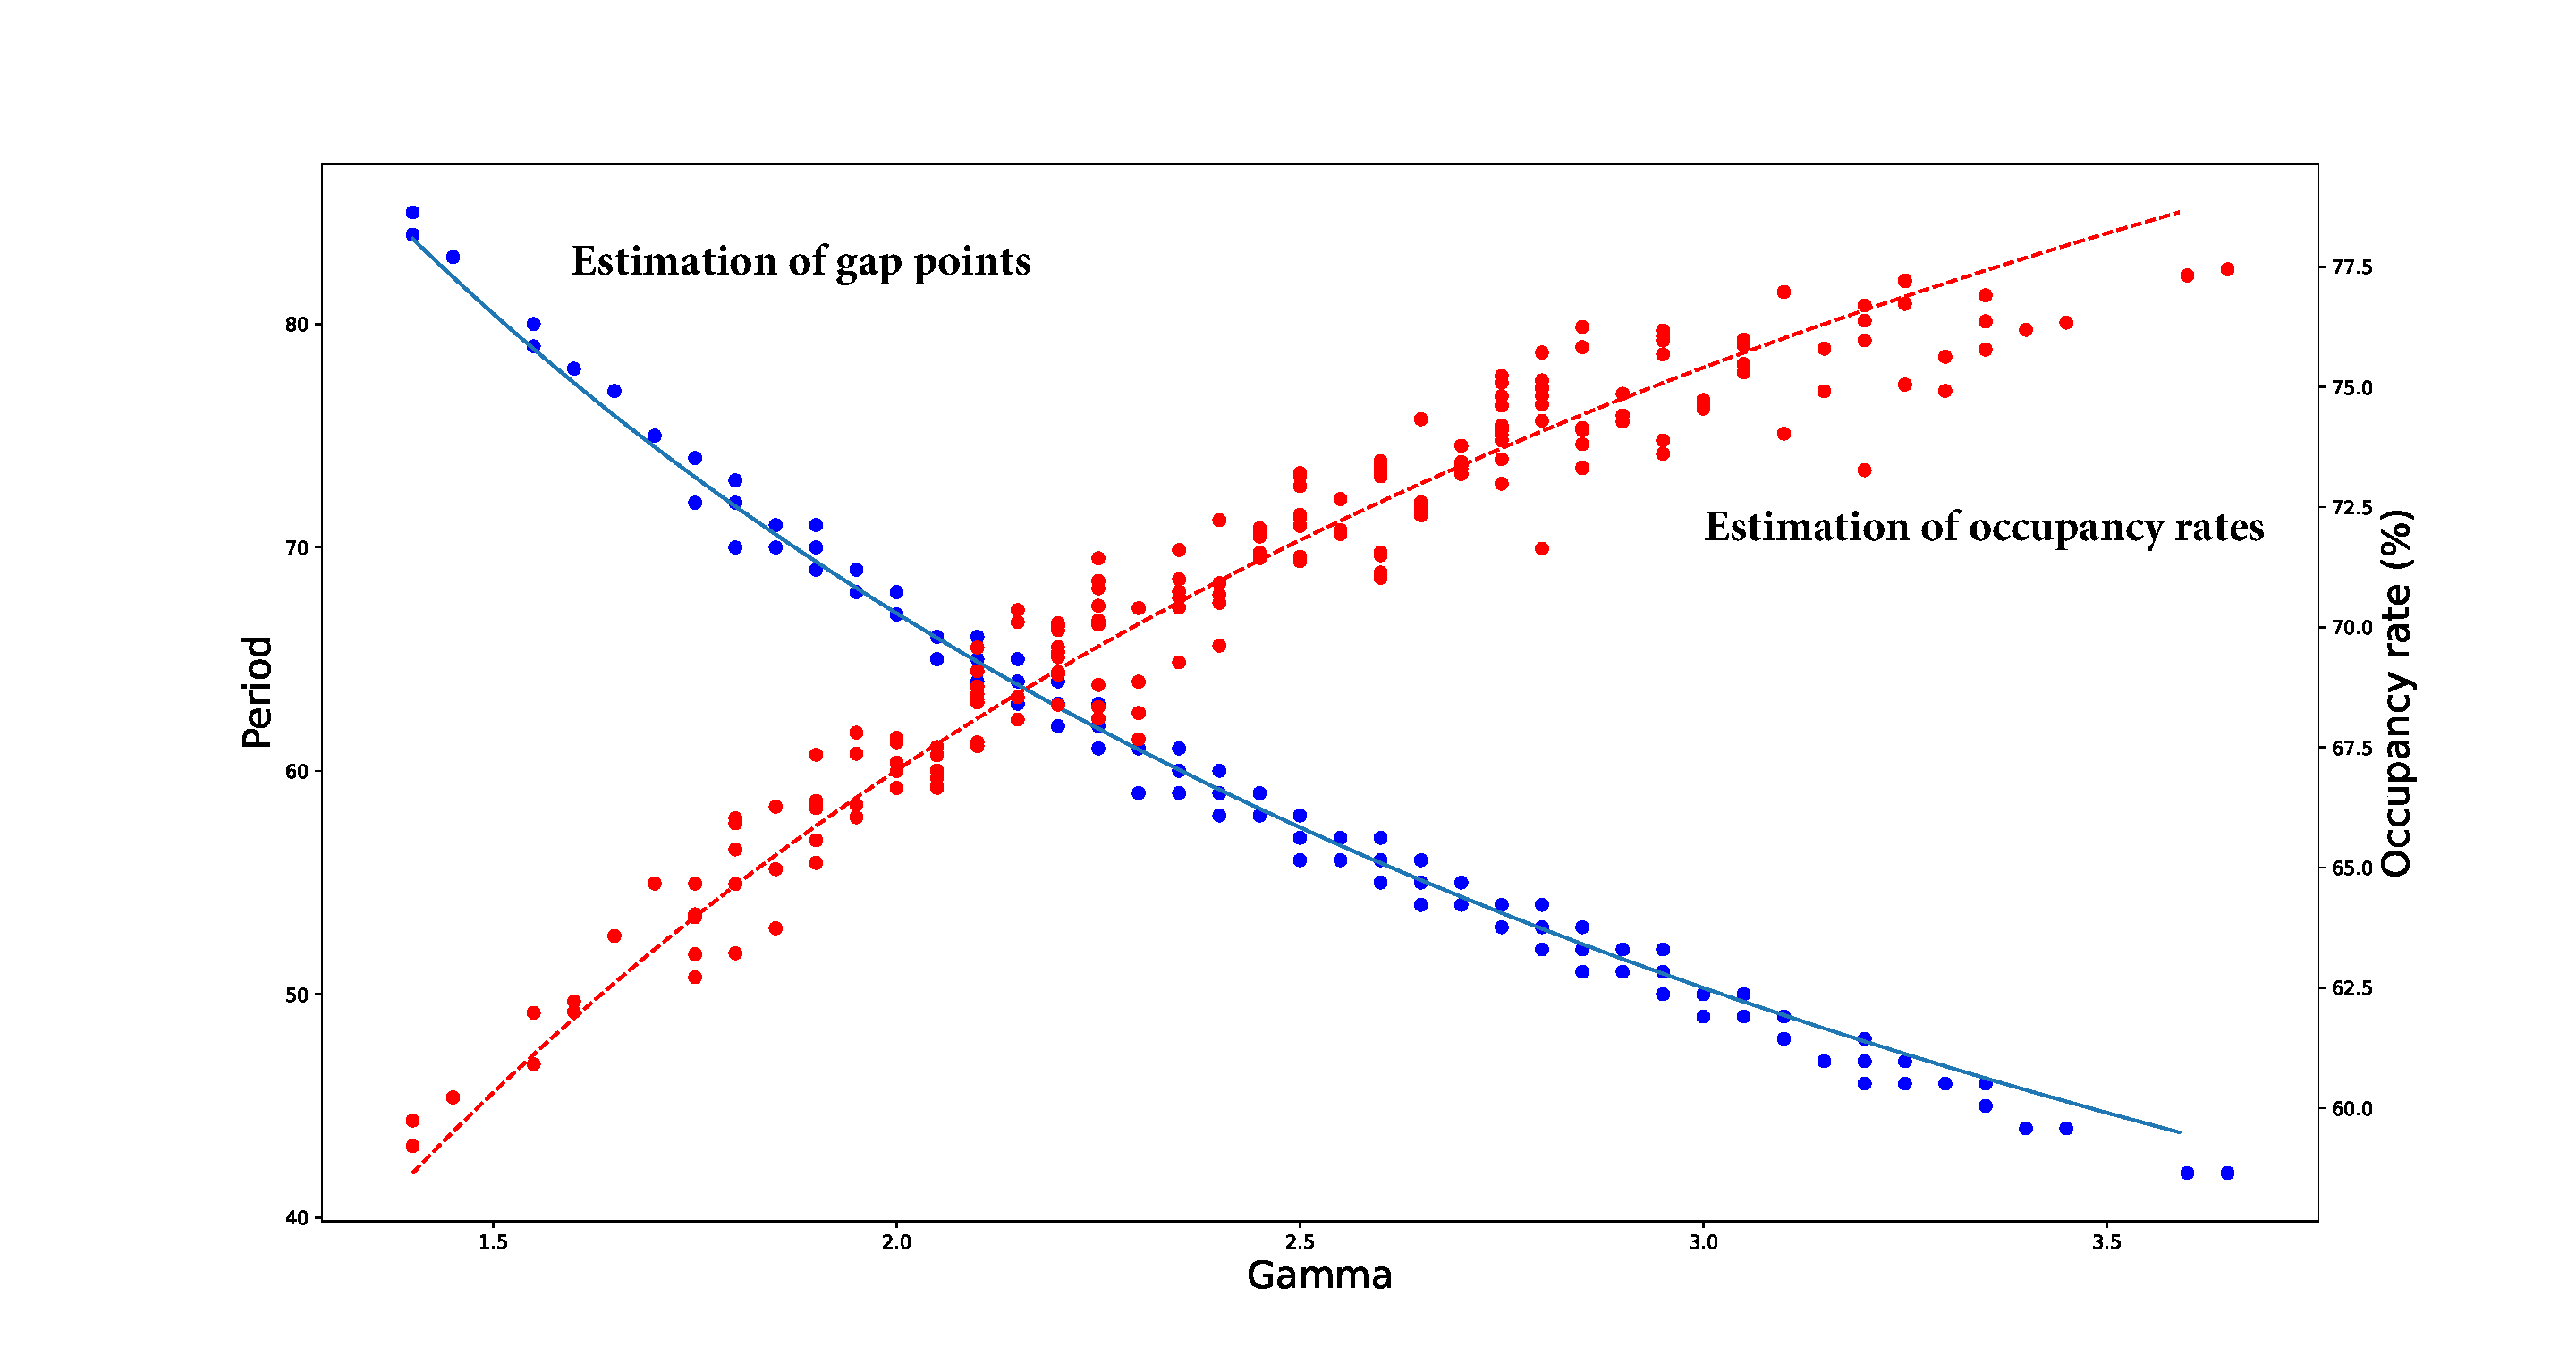
\includegraphics[width=0.95\textwidth]{./Figures/200_random.pdf}
\end{figure}

\subsection{Performance Evaluation Under Varied Constraints}\label{perf_constraints}
To comprehensively evaluate the effectiveness of government policy strictness and venue-specific characteristics, we assess performance using three key metrics: (1) the threshold of request-volume, (2) the threshold of occupancy rate, and (3) the maximum achievable occupancy rate. Our analysis examines how these metrics respond to four critical factors: government-mandated maximum allowable occupancy rates, variations in allowable maximum group sizes, different physical distances ($\delta \in \{1,2\}$) and alternative seat layout configurations.


\subsubsection{Government-mandated maximum allowable occupancy rates}
% add specific government perspective

Government policies may impose a maximum allowable occupancy rate ($\rho^{al}$) to enforce stricter public health measures. The effectiveness of this policy depends on its relationship to two key metrics, threshold of occupancy rate ($\rho^{th}$) and maximum achievable occupancy rate ($\rho^{ac}$).

When $\rho^{al} \leq \rho^{th}$, only the occupancy rate requirement is binding. Once the occupancy rate reaches $\rho^{al}$, all subsequent requests are rejected. When $\rho^{th} \leq \rho^{al} \leq \rho^{ac}$, both maximum allowable occupancy rate and social distancing requirements jointly govern seat assignments. Again, once $\rho^{al}$ is reached, further requests are rejected. When $\rho^{al} \geq \rho^{ac}$ the maximum allowable occupancy rate constraint becomes redundant because the occupancy rate will never exceed $\rho^{al}$ under social distancing.


The conclusion can be summarized in Table \ref{tab_requirement}.
\begin{table}[ht]
  \centering
  \caption{Effectiveness of requirements}\label{tab_requirement}
  \begin{tabular}{ccc}
  \hline
   & Social distancing requirement & requirement of $\rho^{al}$ \\
  %  \cmidrule(r){1-1} \cmidrule(lr){2-2} \cmidrule(lr){3-3} \cmidrule(l){4-4}
  \hline
  $\rho^{al} \leq \rho^{th}$            & Ineffective & Effective \\
  $\rho^{th} \leq \rho^{al} \leq \rho_{ac}$  & Effective   & Effective \\
  $\rho^{al} \geq \rho^{ac}$                  & Effective   & Ineffective \\
   \hline
  \end{tabular}
\end{table}

% This tiered framework enables policymakers to:
% Set $\rho_{al}$ below $\rho_{th}$, for strict capacity control.
% Allow $\rho_{th} \leq \rho_{al} \leq \rho_{ac}$ for graduated reopening.
% Recognize $\rho_{al} \geq \rho_{ac}$ as non-binding for planning purposes.

% Sometimes, the government policy imposes a maximum allowable occupancy rate, $\rho_{al}$, to enforce stricter measures. This rate becomes redundant if it exceeds the maximum achievable rate. When the maximum allowable rate is below the threshold of occupancy rate, only the occupancy rate requirement is effective, rendering the social distancing requirement irrelevant. However, when the maximum allowable rate falls between the threshold of occupancy rate and the maximum achievable rate, both the occupancy rate and social distancing requirements jointly influence seat assignments.

% In the example of Figure \ref{x_period}, the maximum achievable rate is 80.0\%, implying that when the maximum allowable rate exceeds 80.0\%, it is ineffective. The threshold of occupancy rate is 71.8\%, so when the maximum allowable rate is below 71.8\%, only the occupancy rate requirement is effective. When the maximum allowable rate is between 71.8\% and 80\%, both the occupancy rate and social distancing requirements jointly determine seat assignments.


\subsubsection{Different Allowable Maximum Group Sizes and Physical Distances}
When $M$ is restricted at 3, given the probability distribution [0.12, 0.5, 0.13, 0.25], we discard the fourth component and normalize the remaining three components to generate a new probability distribution: [0.16, 0.67, 0.17]. Similarly, when $M =2$, the probability distribution is [0.19, 0.81].
We also consider the impact of different distances. We present the corresponding threshold of request-volume, the threshold of occupancy rate and the maximum achievable occupancy rate in the table below.

\begin{table}[ht]
  \centering
  \caption{Impact of $M$s and $\delta$s}
  \begin{tabular}{ccccc}
  \hline
   $M$  & $\delta$ & $q^{th}$ & $\rho^{th}$ & $\rho^{ac}$ \\
  %  \cmidrule(r){1-1} \cmidrule(lr){2-2} \cmidrule(lr){3-3} \cmidrule(l){4-4}
  \hline
   2 & 1 & 74  & 66.8 \% & 70.0 \% \\
   2 & 2 & 54  & 48.8 \% & 50.0 \% \\ 
   3 & 1 & 68  & 68.3 \% & 75.0 \% \\
   3 & 2 & 53  & 53.1 \% & 60.0 \% \\
   4 & 1 & 57  & 71.8 \% & 80.0 \% \\
   4 & 2 & 47  & 59.2 \% & 70.0 \% \\
   \hline
  \end{tabular}
\end{table}

For fixed $\delta$, as $M$ increases, $\rho^{th}$ increases, while $q^{th}$ decreases according to the estimation. The maximum achievable occupancy rate increases because $\Phi(M, L_j^{0}, \delta)$ is monotonically increasing in $M$.

For fixed $M$, as $\delta$ increases from 1 to 2 seats, both $q^{th}$ and $\rho^{th}$ decrease (consistent with our earlier analysis). The maximum achievable occupancy rate decreases since $\Phi(M, L_j^{0}, \delta)$ is monotonically decreasing in $\delta$.

% We observe that larger group sizes correspond to higher largest occupancy rates under the same seat layout. However, the gap point and occupancy rate for larger group sizes do not necessarily increase correspondingly. The explanation for this is that as larger groups are allowed to be accepted, seat allocation makes it difficult to achieve a full pattern for each row. Thus, there will be a decrease in both gap points and occupancy rates, i.e., the impact of social distancing will manifest at an earlier period.

% The insight is although allowing larger groups will increase the largest occupancy rate, the impact of social distancing will become evident at an earlier period. Specifically, if demand is low or if the managers wish to avoid rejecting a significant number of customers, they can set a smaller group size limit. Conversely, when demand is high, a larger group size limit can be set to accommodate more customers.

% \subsubsection{Different Physical Distances}
% The following figure illustrates the occupancy rate with different physical distances over the period.

% \begin{figure}[h]
%   \caption{Impact of different distances}\label{result_dis}
%   \centering
%     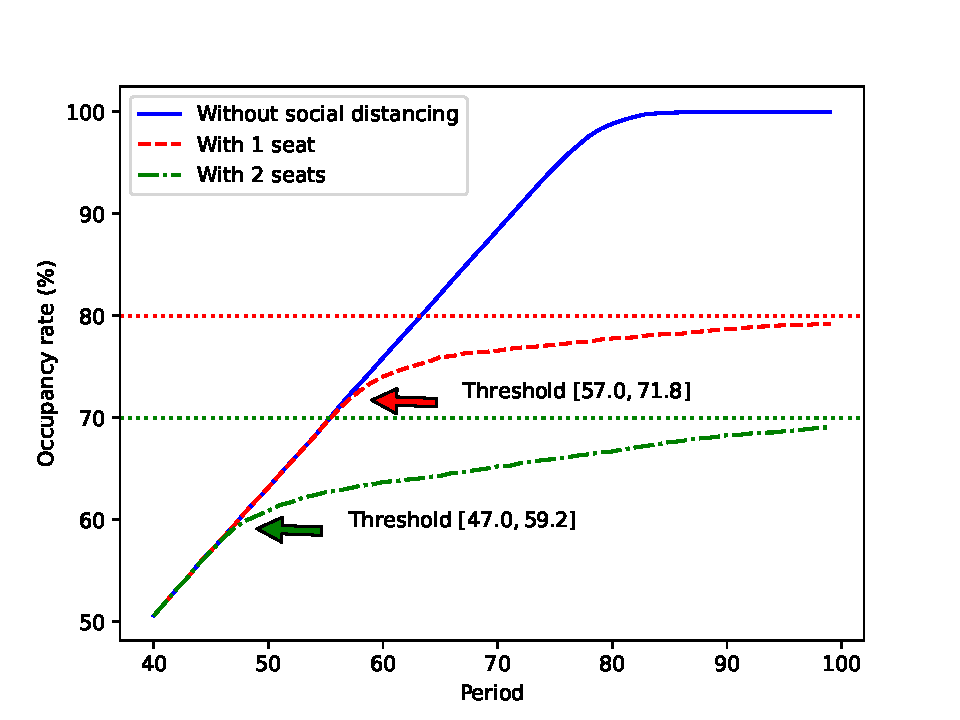
\includegraphics[width=0.7\textwidth]{./Figures/distance_3.pdf}
% \end{figure}

% The threshold of request-volume, the threshold occupancy rate and the maximum achievable occupancy rate are shown in the table below.

% \begin{table}[ht]
%   \centering
%   \caption{Gap points and occupancy rates of $\delta$s}
%   \begin{tabular}{c|ccc}
%   \hline
%    $\delta$  & Gap point & Threshold occupancy rate & Maximum achievable occupancy rate \\
%   %  \cmidrule(r){1-1} \cmidrule(lr){2-2} \cmidrule(lr){3-3} \cmidrule(l){4-4}
%   \hline
%    1 &  57  & 71.76 \% & 80 \% \\
%    2 &  47  & 59.16 \% & 70 \% \\
%    \hline
%   \end{tabular}
% \end{table}



\subsubsection{Alternative Seat Layout configurations}
We experiment with several realistic seat layouts selected from a theater seat plan website, choosing five layouts labeled A, B, C, D, and E. Layouts A, D, and E are approximately rectangular, Layout C is a standard rectangular layout, and Layout B is irregular. In these layouts, wheelchair seats and management seats are excluded, while seats with sufficient space for an aisle are treated as new rows. The specific layouts are detailed in Appendix \ref{appen_3}.

The occupancy rate over demand follows the typical pattern of Figure \ref{occupancy_rate_demand}. The threshold of request-volume, the threshold of occupancy rate and the maximum achievable occupancy rate are also given in the following table. The maximum achievable occupancy rate can be calculated from Proposition \ref{lem_pattern}.

\begin{table}[ht]
  \centering
  \caption{Impact of the layouts}
  \begin{tabular}{cccc}
  \hline
   Layout & $q^{th}$ & $\rho^{th}$ & $\rho^{ac}$ \\
  %  \cmidrule(r){1-1} \cmidrule(lr){2-2} \cmidrule(lr){3-3} \cmidrule(l){4-4}
  \hline
   A & 36 & 72.3 \% & 82.4 \% \\
   B & 38 & 75.8 \% & 84.1 \% \\
   C & 32 & 72.8 \% & 80.0 \% \\
   D & 43 & 74.1 \%  & 83.6 \% \\
   E & 102 & 72.4 \% & 81.7 \% \\
   \hline
  \end{tabular}
\end{table}

Although the layouts may vary in shapes (rectangular or otherwise) and row lengths (long or short), the threshold of occupancy rate and maximum achievable occupancy rate do not exhibit significant differences. Similarly, layouts with varying total seats and rows do not exhibit a clear trend in the threshold of occupancy rate, as estimated based on the analysis.